\documentclass[12pt,UTF8]{ctexbook}
\usepackage{ctex}
\usepackage{graphicx}
\usepackage{float}
\usepackage{wrapfig}
\usepackage{array}
\usepackage[table, dvipsnames, svgnames, x11names]{xcolor}
\usepackage{colortbl}% 
\usepackage{tabularx}
\usepackage{amsmath}
\usepackage{amssymb}
\usepackage{xfrac}
\usepackage{eucal}
\usepackage{titlesec}
\usepackage{amsthm}
\usepackage{tikz-cd}
\usepackage{enumitem}
\usepackage{verbatim}
\usepackage{fontspec,xunicode,xltxtra}
\usepackage{xeCJK} 

\definecolor{gl}{RGB}{246, 252, 240}
\definecolor{gd}{RGB}{236, 244, 230}
\definecolor{bg}{RGB}{242, 244, 228}


\setCJKmainfont[BoldFont=STZhongsong]{STSong}
\setCJKmonofont{simkai.ttf} % for \texttt
\setCJKsansfont{simfang.ttf} % for \textsf
\setlength\parskip{8pt}
\setlength{\fboxsep}{12pt}
\renewcommand\thesection{\arabic{chapter}.\arabic{section}}
\newtheorem{df}{定义}[section] 
\newtheorem{pp}{命题}[section]
\newtheorem{tm}{定理}[section]
\newtheorem{ex}{例子}[section]
\newtheorem{sk}{思考}[section]
\newtheorem{po}{公理}
\newtheorem*{so}{解答}
\newtheorem*{proof2}{证明}
\newtheorem{xt}{习题}[section]
\newtheorem{cor}{推论}[pp]
% 列举环境的行间距
\setenumerate[1]{itemsep=0pt,partopsep=0pt,parsep=0pt,topsep=0pt}
\setitemize[1]{itemsep=0pt,partopsep=0pt,parsep=0pt,topsep=0pt}
\setdescription{itemsep=0pt,partopsep=0pt,parsep=0pt,topsep=0pt}
\setlength{\intextsep}{2pt}%
\setlength{\columnsep}{2pt}%
% 新函数
\renewcommand\parallel{\mathrel{/\mskip-4mu/}}
% 章节字体大小
\titleformat{\section}{\zihao{-2}\bfseries}{ \thesection }{16pt}{}
% 封面
\title{\zihao{0} \bfseries 极简数学·中学篇 \\ 第三册}
\author{\zihao{2} \texttt{大青花鱼}}
% \date{\bfseries\today}
\date{}
% 正文
\begin{document}
\maketitle
\tableofcontents
\newpage

\chapter{相似三角形}
形状一样,大小不同,我们把这样的关系称为相似关系。三角形之间自然也存在相似关系。
如果两个三角形对应的内角都相等或都相反,就说它们\textbf{同角相似}或\textbf{反角相似},统称\textbf{相似}。
一般用$\sim$和$\backsim$表示两个三角形同角和反角相似。如果不要求区分,可以只用$\sim$表示相似。

\begin{wrapfigure}{r}{0.26\textwidth} %this figure will be at the right
    \vspace{-26pt}
    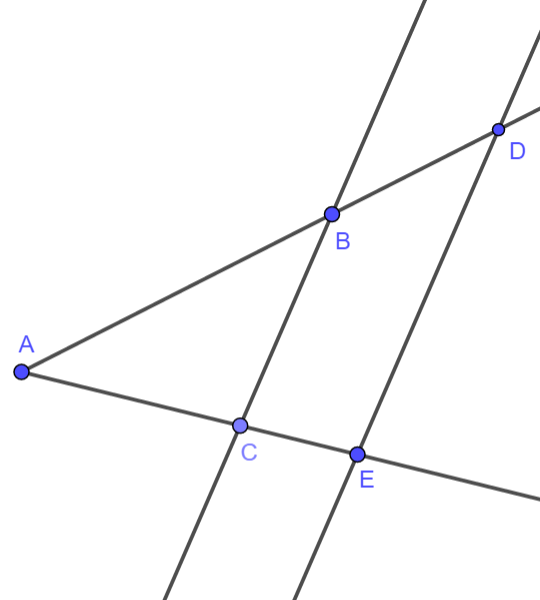
\includegraphics[width=0.26\textwidth]{比例1.png}
\end{wrapfigure}

相似关系比全等关系的要求宽松一些。只要两个三角形全等,它们必然相似。反之,两个三角形相似,它们未必全等。

\section{平行与相似}
我们已经学习过相似关系的基本公理:
\begin{po}{\textbf{放缩公理}}\label{po:6}
    从一点$A$出发的两条射线,每条线上取两点:$B,D$和$C,E$。如果
    $$ \frac{|AB|}{|AD|} = \frac{|AC|}{|AE|},$$
    那么,
    $$ \frac{|AB|}{|AD|} = \frac{|AC|}{|AE|} = \frac{|BC|}{|DE|},$$
    而且$\angle ABC = \angle ADE$,$\angle ACB = \angle AED$。
\end{po}

放缩公理说明,从一点出发的两条射线被两条直线所截,如果截得的线段成相同的比例,那么这两条直线平行。
注意到两条平行线截出了两个三角形:$\triangle ABC$和$\triangle ADE$,它们的三个内角分别相等。
所以$\triangle ABC$和$\triangle ADE$相似。我们把$\frac{|AB|}{|AD|}$称为两者的\textbf{相似比}。

% \begin{wrapfigure}{r}{0.28\textwidth} %this figure will be at the right
%     \vspace{-10pt}
%     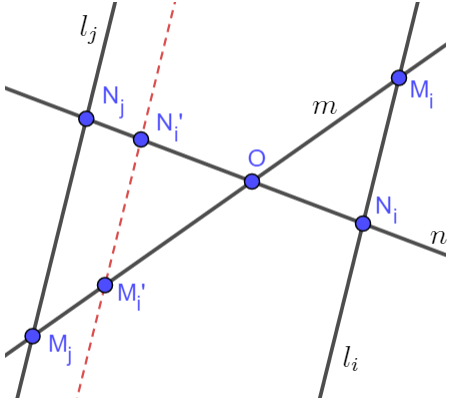
\includegraphics[width=0.28\textwidth]{相似2.png}
% \end{wrapfigure}

反之,通过平行公理可以推出,如果从一点出发的两条射线被两条平行直线所截,那么截得的线段成相同的比例,截得的三角形相似。
甚至,“射线”可以改为“直线”。
% TODO 补上证明

一般来说,如果两个三角形相似,它们对应的边是否成比例呢?
\begin{tm}\label{tm:0-0-1}
    三角形相似,则相等内角的对边成比例。
\end{tm}
\begin{proof2}
    设有三角形:$\triangle ABC \sim \triangle A'B'C'$,即$\angle BAC = \angle B'A'C'$,
    $\angle CBA = \angle C'B'A'$,$\angle BCA = \angle B'C'A'$。在射线$AB$上找一点$D$,使得$|AD| = |A'B'|$,
    在射线$AC$上找一点$E$,使得$|AE| = |A'C'|$。根据“边角边”,$\triangle ADE \simeq \triangle A'B'C'$。
    于是,$\angle DEA = \angle B'C'A' = \angle BCA$。同位角相等,即$DE \parallel BC$。因此
    $$ \frac{|AB|}{|AD|} = \frac{|AC|}{|AE|} = \frac{|BC|}{|DE|}.$$
    即
    $$ \frac{|AB|}{|A'B'|} = \frac{|AC|}{|A'C'|} = \frac{|BC|}{|B'C'|}.$$
    如果$\triangle ABC \backsim \triangle A'B'C'$,同样方法作出的$\triangle ADE \backsimeq \triangle A'B'C'$。
    于是通过类似推理可以得到相同的结论。
\end{proof2}

\section{判定相似关系}
如何判断两个三角形是否相似呢?方法和判断三角形是否全等差不多。

\begin{tm}\label{tm:0-1-0}
    给定$\triangle ABC$和$\triangle A'B'C'$。如果$\angle BAC = \angle B'A'C'$或$\angle BAC = \angle C'A'B'$成立,
    且
    $$ \frac{|AB|}{|A'B'|} = \frac{|AC|}{|A'C'|},$$
    那么$\triangle ABC$和$\triangle A'B'C'$相似。
\end{tm}
这显然是放缩公理的直接应用。
在射线$AB$、$AC$上分别找到点$D$和$E$,使得$|AD| = |A'B'|$,
$|AE| = |A'C'|$,根据“边角边”,$\triangle ADE \cong \triangle A'B'C'$。
于是根据放缩公理,$\triangle ABC$和$\triangle ADE$相似,故而和$\triangle A'B'C'$相似。
我们把这个判断方法也简称为“边角边”。
和全等三角形“边角边”一样,$\angle BAC = \angle B'A'C'$和$\angle BAC = \angle C'A'B'$的情况分别对应同角和反角相似。

判定全等的“角边角”则化为显然的结论:如果两个三角形有两个内角分别相等,则它们相似。

最后,“边边边”则对应定理\ref{tm:0-0-1}的逆命题:
\begin{tm}\label{tm:0-1-1}
    三角形对应的三边成比例,则它们相似。
\end{tm}
\begin{proof2}
    设$\triangle ABC$和$\triangle A'B'C'$满足:
    $$ \frac{|AB|}{|A'B'|} = \frac{|AC|}{|A'C'|} = \frac{|BC|}{|B'C'|}.$$
    在在射线$AB$上找一点$D$,使得$|AD| = |A'B'|$,
    在射线$AC$上找一点$E$,使得$|AE| = |A'C'|$。则
    $$ \frac{|AB|}{|AD|} = \frac{|AB|}{|A'B'|} = \frac{|AC|}{|A'C'|} = \frac{|AC|}{|AE|},$$
    根据放缩公理,
    $$ \frac{|AB|}{|AD|} = \frac{|AC|}{|AE|} = \frac{|BC|}{|DE|},$$
    这说明
    $$ |DE| = \frac{|BC|\cdot |AD|}{|AB|} = \frac{|BC|\cdot |A'B'|}{|AB|} = |B'C'|. $$
    根据“边边边”,$\triangle ADE \cong \triangle A'B'C'$。因此$\triangle ABC \sim \triangle A'B'C'$。
\end{proof2}
我们把这个结论也简称为“边边边”。和判定三角形全等的“边边边”一样,我们无法确定是同角相似还是反角相似。

\section{相似三角形性质与应用}

\begin{wrapfigure}{r}{0.27\textwidth} %this figure will be at the right
    \vspace{-10pt}
    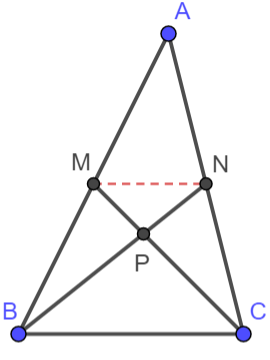
\includegraphics[width=0.27\textwidth]{三角形8.png}
\end{wrapfigure}

相似三角形性质在研究一般三角形性质的时候很有用,因为,我们接下来会看到,三角形里面有很多有趣的相似现象。

\begin{tm}\label{tm:0-2-0}
    三角形顶点和对边中点确定的直线称为该边的中线。设$\triangle ABC$的边$AB$中点为$M$,
    边$AC$的中点为$N$,过$M$的中线$CM$和过$N$的中线$BN$交于一点$P$,则
    $$\frac{|BP|}{|PN|} = \frac{|CP|}{|PM|} = 2.$$
\end{tm}
\begin{proof2}
    从已知条件可以得到:
    $$\frac{|AM|}{|AB|} = \frac{|AN|}{|AC|} = \frac12.$$
    因此,作辅助线$MN$。根据放缩公理,$\triangle AMN \sim \triangle ABC$,相似比为$\frac12$。
    即$|BC| = 2|MN|$。此外还推出$MN \parallel BC$,因此,$\triangle PMN \sim \triangle PCB$。因而有
    $$\frac{|BP|}{|PN|} = \frac{|CP|}{|PM|} = \frac{|BC|}{|MN|} = 2.$$
\end{proof2}

\begin{wrapfigure}{r}{0.27\textwidth} %this figure will be at the right
    \vspace{-10pt}
    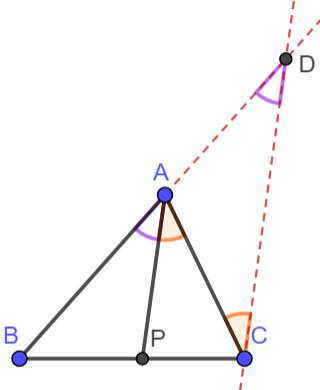
\includegraphics[width=0.27\textwidth]{三角形9.png}
\end{wrapfigure}

$MN$也叫做关于边$BC$的中位线。另外要注意的是:我们只知道点$P$把中线分成长度$2:1$的两段,
并不知道中线本身有多长。

\begin{tm}\label{tm:0-2-1}
    设三角形$\triangle ABC$的内角$\angle BAC$的角平分线交对边于$P$,则
    $$ \frac{|BP|}{|PC|} = \frac{|BA|}{|AC|}.$$
\end{tm}
\begin{proof2}
    过$C$作$AP$的平行线,与射线$BA$交于点$D$。$CD \parallel AP$,所以同位角$\angle BAP = \angle BDC$,
    内错角$\angle PAC = \angle DAC$。而$AP$是角平分线,所以$\angle BAP = \angle PAC$。
    于是$\angle BDC = \angle DAC$,$\triangle ACD$是等腰三角形,$|AC| = |AD|$。\\
    另一方面,$CD \parallel AP$,所以$\triangle BAP \sim \triangle BDC$,因此,
    $$\frac{|BP|}{|PC|} = \frac{|BA|}{|AD|} = \frac{|BA|}{|AC|}.$$
\end{proof2}

\begin{wrapfigure}{r}{0.27\textwidth} %this figure will be at the right
    \vspace{-80pt}
    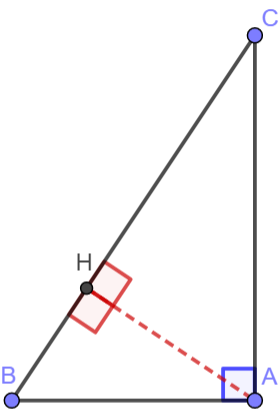
\includegraphics[width=0.27\textwidth]{三角形10.png}
\end{wrapfigure}

我们利用角平分线的性质构造了一个等腰三角形。这是与角平分线相关的问题中常见的思路。
相应地,也可以过$B$作$AC$的平分线,和$AP$交于点$E$,并证明$\triangle ABE$是等腰三角形。

\begin{tm}{\textbf{勾股定理}}\label{tm:0-2-2}
    直角三角形$ABC$中,$\angle A$是直角。则
    $$|AB|^2+|AC|^2 = |BC|^2.$$
\end{tm}
\begin{proof2}
    作$A$到$BC$的垂线,垂足为$H$。$\angle BHA$和$\angle AHC$都是直角。
    $\angle ABH = \angle CBA$,$\angle BHA = \angle BAC$,所以$\triangle HBA \sim \triangle ABC$。
    因此,
    $$ \frac{|BH|}{|BA|} = \frac{|BA|}{|BC|}.$$
    同理,$\triangle HAC \backsim \triangle ABC$。因此,
    $$ \frac{|HC|}{|AC|} = \frac{|CA|}{|BC|}.$$
    这说明
    $$ |BC| = |BH| + |HC| = \frac{|AB|^2}{|BC|} + \frac{|AC|^2}{|BC|}$$
    两边同乘以$|BC|$,就得到
    $$ |BC|^2 = |AB|^2+|AC|^2.$$
\end{proof2}
勾股定理是数学中非常重要的定理,也是非常有名的定理。它的证明方法有四百多种,涉及各种各样的技巧和知识。
勾股定理在西方也称为毕达哥拉斯定理。

\chapter{三角形的四线五心}
证明三角形性质的时候,我们用到了三角形的中点和辅助线。三角形的特殊点和相关辅助线对我们了解三角形的性质是很有帮助的。
接下来我们会介绍四种常见的特殊点和相应的辅助线。它们一般合称为三角形的四线。

\section{垂直平分线和外心}
垂直平分线定理告诉我们,三角形每条边都对应一条称为垂直平分线的直线。这条直线是到它的两个端点距离相等的点的集合,
是过它的中点,且与它垂直的直线。三角形的三边,对应三条垂直平分线。这三条垂直平分线有什么联系呢?

我们先看两条垂直平分线的关系。给定三角形$ABC$,记顶点$A$对边的垂直平分线为$p(A)$,$B$对边的垂直平分线为$p(B)$。
按照定义,$p(A)$垂直于直线$BC$,$p(B)$垂直于直线$AC$。如果$p(A)$和$p(B)$相交于点$O$,那么因为$O$在$p(A)$上,$|OB| = |OB|$;
同理,也有$|OA| = |OC|$。于是$|OA| = |OB|$,$O$也在$C$对边的垂直平分线$p(C)$上。
也就是说,三角形三边的垂直平分线都交于点$O$。

那么,$p(A)$和$p(B)$是否总相交呢?两条直线要么相交,要么平行或重合。
如果$p(A)$和$p(B)$平行或重合,根据垂直定理及推论,直线$BC$和$AC$平行或重合。
因此,要么$A,B,C$共线,这时我们说三角形退化为直线,要么$p(A)$和$p(B)$相交。
\begin{tm}{\textbf{外心定理}}\label{tm:1-0-0}
    (非退化的)三角形三边的垂直平分线交于一点,称为三角形的\textbf{外心}。
\end{tm}
按照定义,外心到三角形三个顶点的距离相同。

\section{垂线和垂心}
\begin{wrapfigure}{r}{0.4\textwidth} %this figure will be at the right
    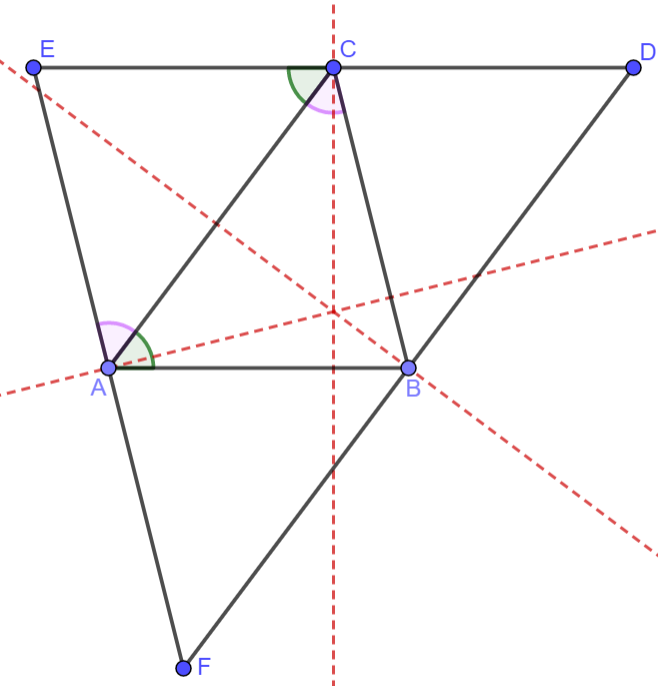
\includegraphics[width=0.4\textwidth]{三角形7.png}
\end{wrapfigure}

垂线定理告诉我们,过三角形每个顶点,都有唯一垂直于对边的直线。
我们把$A$到对边$BC$的垂线记为$h(A)$,$B$到$CA$的垂线记为$h(B)$,$C$到$AB$的垂线记为$h(C)$。
它们也叫三角形的\textbf{高线}。对应的垂足记为$H_A$、$H_B$、$H_C$。
这三条直线有什么关系呢?
\begin{tm}{\textbf{垂心定理}}\label{tm:1-1-0}
    (非退化的)三角形三\\
    边的垂线交于一点,称为三角形的\textbf{垂心}。
\end{tm}
\begin{proof2}
    如右图,过三角形顶点$A,B,C$分别作平行于对边的直线,它们两两相交于$D,E,F$。
    $\angle BAC$和$\angle ECA$是内错角,所以相等。同理,$\angle ACB = \angle CAE$。
    此外$|AC| = |CA|$。因此,根据“角边角”,$\triangle ABC \cong \triangle CEA$。
    于是$|CE| = |AB|$,$|AE| = |BC|$。\\
    类似地,有$\triangle ABC \cong \triangle DCB$,$\triangle ABC \cong \triangle BAF$。
    因此,$|CD| = |AB|$,$|BD| = |AC|$,$|BF| = |AC|$,$|AF| = |BC|$。进而可得,
    $A$是线段$EF$中点,$B$是线段$DF$中点,$C$是线段$DE$中点。垂线$h(A), h(B), h(C)$分别是
    三角形$DEF$三边的垂直平分线。根据外心定理\ref{tm:1-0-0},它们交于一点。
\end{proof2}
\begin{xt}\label{xt:1-1-0}
    \mbox{}\\
    给定三角形$ABC$的垂心$H$,\\
    1. 证明:$B$是三角形$ACH$的垂心。\\
    2. $A,B,C,H$四点之间有什么关系?\\
    过锐角三角形$ABC$的顶点$A$作$BC$的垂线,交$BC$于点$H_A$。\\
    1. 请用$|AH_A|$、$|BC|$和$|H_AC|$表示$|AC|$和$|AB|$。\\
    2. $|AC|^2$和$|AB|^2 + |BC|^2$有什么关系?\\
    3. 如果$\triangle ABC$是钝角三角形,$\angle C$是钝角,你能得到什么结论?\\
    4. 请写出勾股定理的逆命题。它是否成立?
\end{xt}

\section{角平分线、内心和旁心}
\begin{wrapfigure}{r}{0.28\textwidth} %this figure will be at the right
    \vspace{-20pt}
    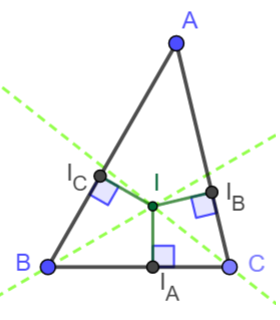
\includegraphics[width=0.28\textwidth]{三角形内心.png}
\end{wrapfigure}
三角形每个内角和外角都有角平分线,分别叫内角平分线和外角平分线。
\begin{tm}{\textbf{内心定理}}\label{tm:1-2-0}
    (非退化的)三角形内角的平分\\
    线交于一点,称为三角形的\textbf{内心}。
\end{tm}
\begin{proof2}
    设$\triangle ABC$的内角:$\angle B$和$\angle C$的平分线交于一点$I$,
    作$I$到三角形三边的垂线,设垂足分别为$I_A$、$I_B$、$Q_C$。
    根据角平分线定理,$|I_AI| = |I_BI|$、$|I_AI| = |I_CI|$。所以$|I_CI| = |I_BI|$,
    根据角平分线定理的逆定理,$I$也在$\angle A$的平分线上。
\end{proof2}

\begin{wrapfigure}{r}{0.28\textwidth} %this figure will be at the right
    \vspace{-25pt}
    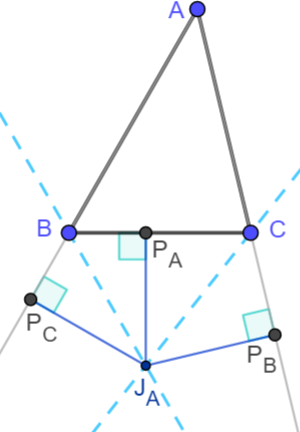
\includegraphics[width=0.28\textwidth]{三角形旁心.png}
\end{wrapfigure}

三角形的内心可以看作到三边距离相等的点。作为对比,外心是到三个顶点距离相等的点。
三角形的内角平分线和外角平分线也有交点。在以上证明的启发下,我们自然也猜测外角平分线有类似的“心”。

\begin{tm}{\textbf{旁心定理 }}\label{tm:1-2-1}
    (非退化的)三角形任一内角\\
    的平分线和另外两个外角的平分线交于一点,称为三\\
    角形的\textbf{旁心}。
\end{tm}
\begin{proof2}
    设$\triangle ABC$的外角:$\angle B$和$\angle C$的平分线交于一点$J_A$,
    作$J_A$到三角形三边所在直线的垂线,设垂足分别为$P_A$、$P_B$、$P_C$。
    根据角平分线定理,$|P_AJ_A| = |P_BJ_A|$、$|P_AJ_A| = |P_CJ_A|$。所以$|P_CJ_A| = |P_BJ_A|$,
    根据角平分线定理的逆定理,$J_A$也在内角$\angle A$的平分线上。
\end{proof2}

三角形每个内角和另外两个外角都可以构造一个旁心,所以,三角形有一个内心和三个旁心。

\begin{wrapfigure}{r}{0.4\textwidth} %this figure will be at the right
    \vspace{-30pt}
    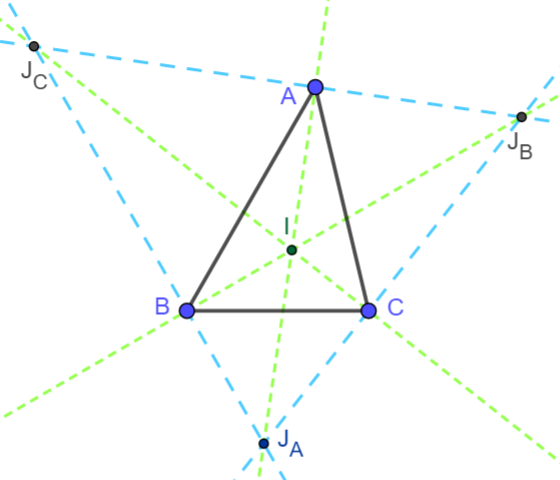
\includegraphics[width=0.4\textwidth]{三角形内心旁心.png}
\end{wrapfigure}

如果我们把三个旁心连成三角形,就会发现,原三角形的顶点在新三角形的边上,
而且恰好是新三角形顶点到对边的高线的垂足。我们把这个新三角形称为原三角形的\textbf{旁心三角形}。

原三角形的内角平分线就是旁心三角形的高线,所以内心作为原三角形内角平分线的交点,
就是旁心三角形的垂心。
\begin{xt}\label{xt:1-2-0}
    \mbox{}\\
    给定三角形$ABC$的内心$I$和旁心$J_A$、$J_B$、$J_C$,证明:\\
    1. $A$在$J_BJ_C$上,$B$在$J_AJ_C$上,$C$在$J_AJ_B$上。\\
    2. $AJ_A \perp J_BJ_C$,$BJ_B \perp J_AJ_C$,$CJ_C \perp J_AJ_B$。\\
    3. $I$是三角形$J_AJ_BJ_C$的垂心。
    % 给定三角形$ABC$的高线$AH_A$、$BH_B$、$CH_C$和垂心$H$,证明:\\
    % 1. $\angle H_BH_AA = \angle AH_AH_C$。\\
    % 2. $H$是三角形$H_AH_BH_C$的内心。
\end{xt}

\section{中线和重心}
\begin{wrapfigure}{r}{0.27\textwidth} %this figure will be at the right
    \vspace{-60pt}
    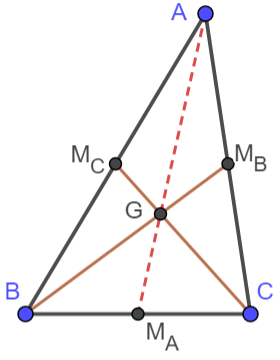
\includegraphics[width=0.27\textwidth]{三角形重心证明.png}
\end{wrapfigure}
三角形每个顶点和对边中点的连线,称为这个顶点到对边的\textbf{中线}或该边上的中线。我们已经学习过
等腰三角形和直角三角形中线的性质。等腰三角形的三条中线交于一点。一般情况下,这件事也成立。

\begin{tm}{\textbf{重心定理}}\label{tm:1-3-0}
    (非退化的)三角形三边上的中
    线交于一点,称为三角形的\textbf{重心}。
\end{tm}
\begin{proof2}
    设$\triangle ABC$三边中点为$M_A$、$M_B$、$M_C$,中线$BM_B$和$CM_C$交于点$G$。
    根据定理\ref{tm:0-2-0},
    $$\frac{|BG|}{|GM_B|} = \frac{|CG|}{|GM_C|} = 2.$$
    也就是说,$G$在线段$BM_B$上,而且$|BG| = \frac23 |BM_B|$。同理,设中线$BM_B$和$AM_A$交于点$G'$。也有:
    $$\frac{|BG|}{|G'M_B|} = \frac{|AG'|}{|G'M_A|} = 2.$$
    $G$和$G'$都在线段$BM_B$上,且$|BG| = \frac23 |BM_B| = |BG'|$。
    这说明$G$和$G'$是同一点,它是$AM_A$、$BM_B$和$CM_C$的公共点。
\end{proof2}
重心的概念有物理的意义。均匀分布的物体受到的重力,可以视为重心受到的重力。
\begin{xt}\label{xt:1-3-0}
    $\triangle ABC$的中线$AM_A$、$BM_B$和$CM_C$交于重心$G$,讨论:\\
    1. $\triangle BGC$的面积和$\triangle ABC$的面积有什么关系?$\triangle BGA$和$\triangle AGC$呢?\\
    2. $\triangle AM_BM_C$的面积和$\triangle ABC$的面积有什么关系?$\triangle BM_AM_C$和$\triangle CM_AM_B$呢?\\
    3. $\triangle GM_BM_C$的面积和$\triangle ABC$的面积有什么关系?$\triangle GM_AM_C$和$\triangle GM_AM_B$呢?\\
    设$\triangle ABC$是等腰三角形,$|AB| = |AC|$,证明:顶点$A$到边$BC$的中线、垂线和$\angle A$的平分线重合。\\
\end{xt}

\chapter{归纳和反证}
严谨的推理和证明是数学研究的基石。漫长的数学研究历史中,人们发明了各种各样的推理和证明技巧。
归纳和反证是两种很有用、很常用的证明技巧。

\section{命题的否定}
命题,就是包含判断的语句。\textbf{命题的否定},是一个和原来的命题矛盾的命题。只要原来的命题是真的,它就是假的。
只要原来的命题是假的,它就是真的。对生活中具体的命题来说,命题的否定可能有多种多样的形式,和使用的语言、文体、措辞都有关系。
数学上,为了方便,我们把命题$p$的否定记为“非$p$”。

判断一个命题是不是命题的否定,可以通过真值表。如果在每种情况下,命题$q$的真值和命题$p$的真值都相反,
那么$q$就是$p$的否定。

对简单判断构成的命题来说,命题的否定取决于全称、有称还是单称。单命题的否定就是它的非命题。
比如:“小明不是校篮球队的队员”的否定是“小明是校篮球队的队员”,“$4$是偶数”的否定是“$4$不是偶数”。
全命题的否定是它的有非命题,有命题的否定是它的全非命题。

为了方便,我们把否定记为$\neg$,比如$p$的否定记为$\neg p$。于是,以上的结论可以写成:
\begin{align}
    \neg  (\forall a\in A, \,\,\, P(a)) &= (\exists a\in A, \,\,\, \neg P(a)), \notag \\
    \neg  (\exists a\in A, \,\,\, P(a)) &= (\forall a\in A, \,\,\, \neg P(a)). \notag
\end{align}

对复合命题,命题的否定涉及到构成复合命题的各个部分。

观察以下真值表,你有什么发现?
\begin{center}
    \begin{tabular}{ p{2em}<{\centering} p{2em}<{\centering} p{4em}<{\centering} p{4em}<{\centering} p{6em}<{\centering} p{6em}<{\centering} }
        \rowcolor{gd} $p$ & $q$ & $p$并且$q$ & $p$或者$q$ & 非$p$并且非$q$ & 非$p$或者非$q$\\ [0.5ex] 
        \noalign{{\color{white}\hrule height 2pt}} % \hline\hline
        \rowcolor{gl} 真 & 真 & 真 & 真 & 假 & 假 \\  
        \noalign{{\color{white}\hrule height 2pt}}% \hline
        \rowcolor{gd} 真 & 假 & 假 & 真 & 假 & 真\\
        \noalign{{\color{white}\hrule height 2pt}}% \hline
        \rowcolor{gl} 假 & 真 & 假 & 真 & 假 & 真\\  
        \noalign{{\color{white}\hrule height 2pt}}% \hline
        \rowcolor{gd} 假 & 假 & 假 & 假 & 真 & 真\\
    \end{tabular}
\end{center}
我们发现,命题$p$和$q$取遍所有可能的情况时,联言命题“$p$并且$q$”和或言命题“非$p$或者非$q$”的真假刚好相反。
同样,或言命题“$p$或者$q$”和联言命题“非$p$并且非$q$”的真假也刚好相反。因此,“$p$并且$q$”的否定是“非$p$或者非$q$”。
“$p$或者$q$”的否定“非$p$并且非$q$”

联言命题的否定,是它各个分支的否定的或言命题;或言命题的否定,是它各个分支的否定的联言命题。

为了方便,我们把“$p$并且$q$”记为$p\wedge q$,把“$p$或者$q$”记为$p\vee q$。于是,上面的规则可以简单记为:
$$ \neg (p \wedge q) = (\neg p) \vee (\neg q), \quad \neg (p \vee q) = (\neg p) \wedge (\neg q). $$

观察以下真值表,你有什么发现?
\begin{center}
    \begin{tabular}{ p{2em}<{\centering} p{2em}<{\centering} p{4em}<{\centering} p{5em}<{\centering} p{5em}<{\centering} p{6em}<{\centering} }
        \rowcolor{gd} $p$ & $q$ & 若$p$则$q$ & 若$p$则非$q$ & $p$而且非$q$ & 若非$p$则非$q$\\ [0.5ex] 
        \noalign{{\color{white}\hrule height 2pt}} % \hline\hline
        \rowcolor{gl} 真 & 真 & 真 & 假 & 假 & 真 \\  
        \noalign{{\color{white}\hrule height 2pt}}% \hline
        \rowcolor{gd} 真 & 假 & 假 & 真 & 真 & 真\\
        \noalign{{\color{white}\hrule height 2pt}}% \hline
        \rowcolor{gl} 假 & 真 & 真 & 真 & 假 & 假\\  
        \noalign{{\color{white}\hrule height 2pt}}% \hline
        \rowcolor{gd} 假 & 假 & 真 & 真 & 假 & 真\\
    \end{tabular}
\end{center}
我们发现,命题$p$和$q$取遍所有可能的情况时,假言命题“若$p$则$q$”的否定不是“若$p$则非$q$”,也不是“若非$p$则非$q$”,
而是“$p$而且非$q$”。为了方便,我们把“若$p$则$q$”记为$p \Rightarrow q$,于是:
$$ \neg (p \Rightarrow q) = p \wedge (\neg q).$$

\begin{sk}\label{sk:2-0-0}
    选言命题“要么$p$,要么$q$”、必要条件假言命题“只有$p$,才有$q$”和充分必要条件假言命题“$p$当且仅当$q$”的否定分别是什么?
\end{sk}

\begin{xt}\label{xt:2-0-0}
    以下例子中,后面的命题是前面的命题的否定吗?\\
    1. “如果不下雨,我就把印章送过去”和“如果下雨,我就把印章送过去”。\\
    2. “如果$n$是$3$的倍数,那么$m$是$7$的倍数”和“$n$是$3$的倍数,而且$m$不是$7$的倍数”。\\
    3. “如果旅馆不提供早餐,那么有些队员不愿意参加秋季合宿训练计划”和“旅馆不提供早餐,而且有些队员愿意参加秋季合宿训练计划”。\\
    4. “线段$AB$上有些点既是中线上的点,也是垂直平分线上的点”和“线段$AB$上所有点既不是中线上的点,也不是垂直平分线上的点”。
\end{xt}

\section{反证法}
反证法,也称为归谬法,是一种古老的推理方法。为了论证某个命题是真的,我们先假设它是假的,然后展开推理,直到出现矛盾。
正确的推理得到了矛盾,就说明我们最初的假设是有问题的,某论断不是假的,因此是真的。同样,为了论证某个命题是假的,
我们也可以假设它是真的,推理得到矛盾,从而说明判断是假的。

实际操作中,为了论证某个命题是真的(或假的),我们一般假设命题的否定是真的(或假的)。命题的否定,
真假和原命题相反,所以从命题的否定为真(或假)推出矛盾,就说明原命题为真(或假)。

\begin{ex}\label{ex:2-0-0}
    如果任一整数$n$的平方是偶数,那么$n$也是偶数。
\end{ex}
\begin{proof2}
    使用反证法。命题“如果任一整数$n$的平方是偶数,那么$n$也是偶数”的否定是“至少有一个整数$n$,它的平方是偶数,并且它不是偶数”。
    为了证明原命题是真的,我们假设它的否定是真的,然后推理得到矛盾。\\
    反设至少有一个整数$n$的平方是偶数,而且$n$不是偶数。于是$n$是奇数,可以写成:
    $$ n = 2k+1.$$
    其中$k$是整数。于是:
    $$ n^2 = (2k+1)^2 = 4k^2 + 4k + 1.$$
    即
    $$ n^2 = 4k(k+1)+1.$$
    于是$n^2$是奇数。但$n^2$是偶数。这就产生了矛盾!
    这说明原命题的否定“至少有一个整数$n$,它的平方是偶数,并且它不是偶数”是假的,因此原命题是真的。
\end{proof2}

\begin{ex}\label{ex:2-0-1}
    证明:\\
    任何有理数的平方都不是$2$。
\end{ex}
\begin{proof2}
    使用反证法。命题“任何有理数的平方都不是$2$”的否定是“至少有一个有理数的平方是$2$”。
    为了证明原命题是真的,我们假设它的否定是真的,然后推理得到矛盾。\\
    反设至少有一个有理数的平方是$2$,设某个有理数$r$的平方等于$2$。把$r$写成既约分数:$\frac{p}{q}$。
    $$ \left(\frac{p}{q}\right)^2 = 2$$
    所以,
    $$ p^2 = 2q^2.$$
    于是$p^2$是偶数,因此$p$也是偶数。把$p$写成$p = 2m$,其中$m$是整数,于是:
    $$ 4m^2 = 2q^2.$$
    即
    $$ q^2 = 2m^2.$$
    于是$q^2$也是偶数,这说明$q$是偶数。因此$p$和$q$都是偶数。但$\frac{p}{q}$是既约分数。这就产生了矛盾!
    这说明原命题的否定“至少有一个有理数的平方是$2$”是假的,因此原命题是真的。
\end{proof2}

\begin{wrapfigure}{r}{0.27\textwidth} %this figure will be at the left
    \vspace{10pt}
    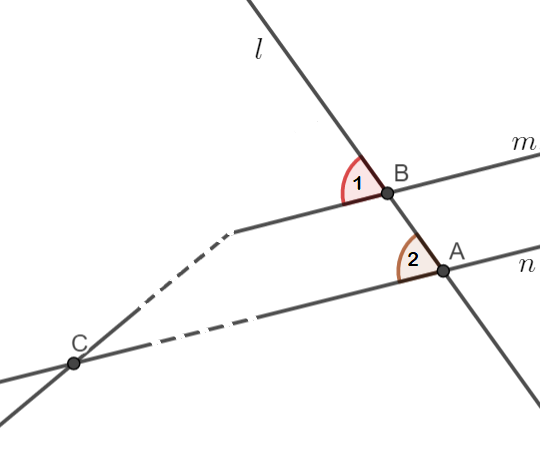
\includegraphics[width=0.27\textwidth]{反证法1.png}
\end{wrapfigure}
当原命题是“任何”、“不存在”这种全判断的时候,它的否定是“至少有一个”这种有判断。这时,使用反证法就可以对这个“有一个”
的特例进行论证,非常方便。

\begin{tm}\label{tm:2-0-0}
    两条直线$m,n$交另一条直线$l$于两点。如果同位角相等,那么$m,n$平行。
\end{tm}
\begin{proof2}
    使用反证法。命题“如果同位角相等,那么$m,n$平行”的否定是“有一对同位角相等,而且$m,n$不平行”。
    为了证明原命题是真的,我们假设它的否定是真的,然后推理得到矛盾。\\
    反设有一对同位角$\angle 1$和$\angle 2$相等,而且$m,n$不平行。设$m,n$的交点$C$在点$A$的一侧(如右图)。
    $\angle ACB + \angle 2$等于$\angle 1$的补角。但$\angle 1 = \angle 2$,
    所以$\angle ACB = 0^\circ$,这说明$m$和$n$重合而非平行。\\
    这就产生了矛盾!\\
    如果交点$C$在点$A$另一侧,通过类似推理可同样推出矛盾。\\
    这说明原命题的否定“有一对同位角相等,而且$m,n$不平行”是假的,因此原命题是真的。
\end{proof2}
反证法的好处在于,通过假设命题的否定为真,我们多了一个用来推理的条件。

\begin{xt}
    用反证法证明:\\
    1. 如果任一整数$n$的立方是奇数,那么$n$也是奇数。\\
    2. 所有奇数的平方除以$8$都余$1$。\\
    动手做:\\
    补全定理\ref{tm:2-0-0}中根据“交点$C$在点$A$另一侧”推出矛盾的过程。
\end{xt}

\section{归纳法}
\begin{sk}\label{sk:2-2-0}
    观察并验证以下等式,你有什么发现?\\
    1. $1 + 3 = \frac12(3^2 - 1)$,$1 + 3 + 9 = \frac12(3^3 - 1)$,$1 + 3 + 9 + 27 = \frac12(3^4 - 1)$。\\
    2. $1 = \frac12(1+1)$,$1 + 2 = \frac22(1 + 2)$,$1 + 2 + 3 = \frac32(1 + 3)$。\\
    3. $\frac13 + \frac14 + \frac15 + \frac16 > \frac{9}{10}$,$\frac14 + \frac15 + \cdots + \frac{1}{9} > \frac{9}{10}$,
    $\frac15 + \frac16 + \cdots + \frac{1}{12} > \frac{9}{10}$。    
\end{sk}
从纷乱繁杂的事物中发现规律,是人类认识自然、改造自然的活动中不可缺少的一环。
归纳,就是试图用简单的规则概括已知的现象。比如,上面第一个例子中,我们可以归纳出这样的规律:
$$ \forall n \in \mathbb{N}, \,\,\, 1 + 3 + 3^2 + \cdots + 3^n = \frac{3^{n+1} - 1}{2}. $$
第二个例子中,我们可以归纳出:
$$ \forall n \in \mathbb{Z}^+, \,\,\, 1 + 2 + \cdots + n = \frac{n(n+1)}{2}. $$
第三个例子中,我们可以归纳出:
$$ \forall n \in \mathbb{Z}^+, \,\,\, \frac{1}{n+1} + \frac{1}{n+2} + \cdots + \frac{1}{3n} > \frac{9}{10}. $$
归纳得到的规律,并不总是正确的。比如,把$n=1$代入我们从第三个例子中归纳出来的不等式:
$$ \frac12 + \frac13 > \frac{9}{10}.$$
这个结论是错的。

怎样正确地归纳事物的规律呢?或者说,什么时候,我们可以确信归纳出的规律是正确的呢?
在漫长的数学研究中,人们认识到:
\begin{po}{\textbf{归纳公理}}
    设$P(n)$是一个含变量的命题,变量$n$可以是任意自然数。如果$P$满足以下两个条件:\\
    1. $P(0)$成立。\\
    2. 对每个自然数$n$,只要$P(n)$成立,$P(n+1)$就成立。\\
    那么,$P(n)$对任意自然数$n$都成立。
\end{po}
使用归纳公理的证明,也叫做用(数学)归纳法证明。用“数学”两个字,是为了和日常生活中凭有限经验归纳的做法区别开来。

以上三个例子中的规律,如何用归纳公理来论证呢?我们分别来写出过程。
\begin{proof2}{\textbf{第一个例子 }}
    命题$P(n)$:
    $$ 1 + 3 + 3^2 + \cdots + 3^n = \frac{3^{n+1} - 1}{2}. $$
    按照归纳公理,要论证命题对任意自然数$n$都成立,我们分别验证两个条件:\\
    1. $P(0)$可以写成:$1 = \frac{3 - 1}{2}$,显然成立。\\
    2. 假设$P(n)$对某个自然数$n$成立,我们来证明$P(n+1)$成立。\\
    $P(n+1)$可以写成:
    $$ 1 + 3 + 3^2 + \cdots + 3^{n+1} = \frac{3^{n+2} - 1}{2}. $$
    由于$P(n)$成立,$(1)$式左边的前$n+1$项可以写成$\frac{3^{n+1} - 1}{2}$,于是两边同时减去这一项,得到:
    \begin{align}
        3^{n+1} &= \frac{3^{n+2} - 1}{2} - \frac{3^{n+1} - 1}{2} \notag \\
        &= \frac{3\cdot 3^{n+1}}{2} - \frac{3^{n+1}}{2} \notag \\
        &= \frac{3\cdot 3^{n+1} - 3^{n+1}}{2} \notag \\
        &= \frac{2 \cdot 3^{n+1}}{2} = 3^{n+1} \notag
    \end{align}
    显然成立。因此,根据归纳公理,$P(n)$对任意自然数$n$都成立。    
\end{proof2}
我们可以看到,论证的时候,我们分别验证归纳公理要求的两个条件成立。从复杂的代数式到显然成立的等式,
我们用到了变量代换和因式分解的技巧。

\begin{proof2}{\textbf{第二个例子 }}
    命题$P$只对正整数有定义,所以我们要证明$P(n)$对所有正整数$n$成立。
    为此,我们稍微改变一下论证方式。\\
    命题$P(n)$:
    $$ 1 + 2 + \cdots + n = \frac{n(n+1)}{2}. $$
    按照归纳公理,要论证命题对任意自然数$n$都成立,我们分别验证两个条件:\\
    1. $P(1)$可以写成:$1 = \frac{1(1+1)}{2}$,显然成立。\\
    2. 假设$P(n)$对某个自然数$n$成立,我们来证明$P(n+1)$成立。\\
    $P(n+1)$可以写成:
    $$ 1 + 2 + \cdots + (n+1) = \frac{(n+1)(n+2)}{2}.  $$
    由于$P(n)$成立,$(1)$式左边的前$n$项可以写成$\frac{n(n+1)}{2}$,于是两边同时减去这一项,得到:
    \begin{align}
        n+1 &= \frac{(n+1)(n+2)}{2} - \frac{n(n+1)}{2} \notag \\
        &= \frac{n+1}{2}\left(n+2 - n\right) \notag \\
        &= \frac{n+1}{2} \cdot 2 = n+1 \notag
    \end{align}
    显然成立。因此,根据归纳公理,$P(n)$对任意正整数$n$都成立。    
\end{proof2}

\begin{proof2}{\textbf{第三个例子 }}
    命题$P(n)$:
    $$ \frac{1}{n+1} + \frac{1}{n+2} + \cdots + \frac{1}{3n} > \frac{9}{10}. $$
    我们已经验证过,$P(1)$不成立。现在利用归纳公理证明$P(n)$对大于等于$2$的自然数成立。
    为此,我们稍微改变一下论证方式。\\
    要论证命题对任意大于等于$2$的自然数$n$成立,我们分别验证两个条件:\\
    1. $P(2)$可以写成:
    $$\frac13 + \frac14 + \frac15 + \frac16 > \frac{9}{10}.$$
    计算可知等式左边等于$\frac{19}{20} > \frac{9}{10}$,因此$P(2)$成立。\\
    2. 假设$P(n)$对某个自然数$n$成立,我们来证明$P(n+1)$成立。\\
    $P(n+1)$可以写成:
    $$ \frac{1}{n+2} + \frac{1}{n+3} + \cdots + \frac{1}{3n+3} > \frac{9}{10}. $$
    由于$P(n)$成立,我们试着把上式左边用$P(n)$有关的式子表达出来,我们发现
    \begin{align}
        \frac{1}{n+2} + \frac{1}{n+3} + \cdots + \frac{1}{3n+3} =& \frac{1}{n+1} + \frac{1}{n+2} + \cdots + \frac{1}{3n} \notag \\
        &+ \frac{1}{3n+1} + \frac{1}{3n+2} + \frac{1}{3n+3} - \frac{1}{n+1} \notag 
    \end{align}
    而
    \begin{align}
        \frac{1}{3n+1} + \frac{1}{3n+2} + \frac{1}{3n+3} - \frac{1}{n+1} &>  \frac{1}{3n+3} + \frac{1}{3n+3} + \frac{1}{3n+3} - \frac{1}{n+1} \notag \\
        = \frac{3}{3n+3} - \frac{1}{n+1} = 0. \notag 
    \end{align}
    这说明:
    $$ \frac{1}{n+2} + \frac{1}{n+3} + \cdots + \frac{1}{3n+3} > \frac{1}{n+2} + \frac{1}{n+3} + \cdots + \frac{1}{3n}. $$
    $P(n)$告诉我们,上式右边大于$\frac{9}{10}$,所以上式左边也大于$\frac{9}{10}$。也就是说,$P(n+1)$成立。\\
    因此,根据归纳公理,$P(n)$对任意大于等于$2$的自然数$n$都成立。    
\end{proof2}
从第二、第三个例子可以看出,归纳公理可以换个“开头”使用。为什么可以这么做呢?让我们来理解归纳公理是如何告诉我们$P(n)$对
任意自然数$n$都成立的。

举例来说,我们知道$P(0)$成立,并且只要$P(n)$成立,$P(n+1)$就成立。现在我们想知道$P(100)$为何成立。
论证过程是这样的:只要$P(n)$成立,$P(n+1)$就成立,而$P(0)$成立,所以$P(1)$也成立。接下来,既然$P(1)$成立,
我们又可以得到$P(2)$成立。以此类推,经过$100$次这样的推理,我们就知道,根据$P(99)$成立,有$P(100)$成立。

使用归纳公理,就好比跑步。第一个条件告诉我们从哪里出发,第二个条件告诉我们,可以一步一步跑下去。第二、第三个例子的证明里,
我们换了一个“起跑线”,但论证了每步都能接到下一步。于是,我们可以从$1$或$2$出发,“跑”到每个大于等于$2$的自然数$n$那里去。

\section{无穷}
做整数除法的时候,我们会遇到两种情况:除得尽和除不尽。列出竖式后,我们用被除数减去除数和商的积,得到余数。
如果某次得到的余数是$0$,就说除法除得尽。如果每次余数都不是$0$,我们就说除法除不尽。我们可以不断按照竖式除法的规则求余数,
但这个过程是无穷无尽的。

夜晚,仰望星空的时候,我们说星星是数不尽的,星星离我们无限遥远。郊游时,看着满地的鲜花,我们说花儿是数不完的。
是因为星星和花朵的数量太多,数起来太费时间,还是因为它们不可能数得完?是因为星星和我们的距离太远,没有测量的办法,
还是因为它们不可能被测量出来?多、远、大、久这些概念,是否有尽头?我们日常形容多、远、大、久等概念的时候,会用“无限”、
“无穷”、“无尽”这样的词来修饰,以表达夸张。到底“无限”、“无穷”、“无尽”是什么意思呢?

为了好理解,我们用数数作为例子:从$1$开始,每次加$1$,也就是$1,2,3,\cdots$这么数下去。会不会到了某一步,我们无法再数下去呢?

如果要数$1$到$1,0000$,那么在第$1,0000$步,我们无法再进行下去了,因为$10,0001$不在里面。
如果要数$1$到$10,0000,0000$,那么在第$10,0000,0000$步,我们无法再进行下去了,因为$10,0000,0001$不在里面。

一般来说,如果要数的是前$n$个正整数,那么在第$n$步,我们就无法进行下去了,因为$n+1$不在里面。

但是,如果要数的是全体正整数,那么我们可以一直进行下去。因为每个正整数$n$后面的数:$n+1$都是正整数。
全体正整数和前$10,0000$个正整数、前$10,0000,0000$个正整数或前$n$个正整数不一样。

数学上,我们将数量分为两类。一类称为“有限”或“有穷”,一类称为“无限”或“无穷”。前$10,0000$个正整数、前$1000,0000$个正整数、
前$n$个正整数这样的集合是有限或有穷的。全体正整数、全体自然数是无限或无穷的。

我们用数数原则判别集合有穷还是无穷。一开始,所有元素都是没数过的。我们对集合重复做数数的动作:每一步,选择一个没数过的元素,
把它标记为数过的。我们简称这个元素被数到了。每个元素至多被数到一次,从没数过变为数过的。如果不论依照什么规则选取,
数数过程都会因为没有没数过的数而停止,就说集合是有穷的,或集合元素的个数是有穷的。如果依照某个规则,数数过程不会停止,
就说集合是无穷的,或集合元素的个数是无穷的。

概括来说,数得尽的集合是有穷的,数不尽的集合是无穷的。

前面我们给正整数设计的数数规则就是一种不会停止的规则:选择上次数到的数加$1$得到的数。一方面,按照这个规则,
每次数到的数总是数过的数里最大的。另一方面,正整数加$1$总是正整数,所以按照规则,用上次数到的数加$1$就得到一个没数过的正整数。
按照数数原则,我们可以判定:全体正整数是无穷的。

依照同一个规则,我们也可以判定:全体自然数是无穷的。

对于前$n$个自然数的集合,我们可以证明它是有穷的。

记前$n$个自然数的集合为$X_n$,数数过程中,记第$i$步结束后所有没数过的数的个数为$G(i)$。
记一开始所有没数过的数的个数为$G(0)$,则$G(0) = n$。无论用什么规则,每一步结束后,没数过的数都少了一个,
即$G(i+1) = G(i) - 1$。于是,$G(n) = G(0) - n = 0$。第$n$步后,不再有没数过的数,数数过程只能停止。
也就是说,$X_n$是有穷的。

要注意的是,数数原则并不总要求每个数都被数过。如果集合是有穷的,按照定义,停止的时候所有的书都被数过。
如果集合是无穷的,那么由于数数过程不会停止,不一定每个数都被数过。比如,我们按照每次加$2$的方式给全体正整数的集合数数:
$1,3,5,\cdots$。这个过程不会停止,但偶数永远不会被数到。

\begin{sk}
    全体整数是否是无穷的?全体有理数呢?你可以总结出什么规律?
\end{sk}

\chapter{根式和实数}

\section{方根}
减法是加法的逆运算,除法是乘法的逆运算,乘方有没有逆运算呢?

$3^2 = 9$,而$9$通过乘$2$次方的逆运算得到$3$。这个运算称为开$2$次方或开平方。

\textbf{开方}是乘方的逆运算。已知一个数的乘方和相应的指数,开方就得到原来的底数。
开方的结果称为\textbf{方根}。一个数开几次方,就得到几次方根。

开$1$次方得到的是自己。开$2$次方也叫开平方,结果叫平方根。开$3$次方也叫开立方,结果叫立方根。
一般来说,开$n$次方的结果叫$n$次方根。一般用$\sqrt[n]{\cdot}$表示开$n$次方运算。比如,
$5$开$3$次方记为$\sqrt[3]{5}$。为了方便,$n=2$时,一般忽略$\sqrt[2]{x}$中的$2$,直接记为$\sqrt{x}$。

开方是映射吗?我们知道$3^2 =9$,但同时也有$(-3)^2 =9$,那么可不可以说$9$开平方得到$-3$呢?

为了让开方成为映射,我们约定:\textbf{方根总是正数}。这样,开方运算就定义了一个映射。

当$n$是偶数的时候,$n$次乘方运算的结果总大于等于零。因此,只有大于等于零的数可以开偶数次方,
负数无法开偶数次方。由于互为相反数的偶数次方相等,开偶数次方运算定义的映射不是一一映射。

当$n$是奇数的时候,$n$次乘方运算的结果可以大于或小于零,因此,正数和负数都可以开奇数次方。
互为相反数的奇数次方也互为相反数。最后,开奇数次方运算定义的映射是一一映射。

指数的加减意味着乘方的乘除,那么指数的乘除意味着什么呢?

考虑$2^{3\times 2} = 2^6$,$3\times 2 = 3 + 3$,于是$2^6 = 2^3 \times 2^3 = \left(2^3\right)^2$。

指数相乘表示乘方的乘方。比如,$2$的$3\times 2$次方等于$2$的$3$次方的$2$次方。
乘法满足交换律,故而$2$的$3$次方的$2$次方也等于$2$的$2$次方的$3$次方。

$4^{3\div 2}$意味着什么呢?

$3\div 2 \times 2 = 3$,所以我们希望$4^{3\div 2 \times 2} = 4^3$,也就是说,
$\left(4^{3\div 2}\right)^2 = 4^3$。
或者说,我们定义$4^{3\div 2}$为$4$的$3$次方再开$2$次方。
这样,我们可以定义一个数的分数次方。

显然,分数次方也不总是存在的,比如$4^{3\div 2}$之所以存在,是因为$4$的$3$次方大于等于零,可以开平方。
如果把$4$改为$-4$,$-4^{3\div 2}$是无法定义的。但如果把$2$换成某个奇数,比如$5$,那么$-4^{3\div 5}$是有定义的。

\begin{sk}\label{sk:3-0-0}
    $n$是奇数时,证明:\\
    1. 如果有理数$a > b$,那么$a^n > b^n$。\\
    2. 给定有理数$a, b$。如果$a^n > b^n$,那么$a > b$。\\
    3. 定义域为$\mathbb{Q}$的函数$x \mapsto \sqrt[n]{x}$是一一映射。\\
    想一想:\\
    $(-3)^{2\div 2}$有意义吗?$n$为奇数和偶数时,$x \mapsto \sqrt[n]{x^n}$分别是怎样的函数?
\end{sk}

\section{无理数和实数}
学习反证法的时候,我们证明了这样一个结论:任何有理数的平方都不是$2$。
而上一节中,我们定义了开平方的运算。$2$开平方的结果记为$\sqrt{2}$,
于是我们有结论:$\sqrt{2}$不是有理数。

另一方面,$\sqrt{2}$是有意义的。勾股定理告诉我们,直角边长为$1$的等腰直角三角形,斜边长的平方等于$1^2+1^2=2$,
因此斜边长是$\sqrt{2}$。也就是说,等腰直角三角形斜边长度和直角边长度之比总是$\sqrt{2}$。

我们把能够表示为长度的数称为(正)实数。或者说,原点到数轴上任一点的距离(按正方向标记正负)构成的集合,称为\textbf{实数}。
实数集合一般记为$\mathbb{R}$。
$\sqrt{2}$能够表示为长度或两点间的距离,所以$\sqrt{2}$是实数。但$\sqrt{2}$不是有理数。我们把这样的实数叫做\textbf{无理数}。

无理数有哪些呢?按照证明\ref{ex:2-0-1}的思路,只要自然数$n$不是完全平方数,$\sqrt{n}$总是无理数。另外,有理数之间的加减乘除总是有理数,所以:
\begin{tm}\label{tm:3-1-0}
    任一无理数和任何有理数进行有限次加减乘除(不包括乘以$0$),得到的结果仍然是无理数。
\end{tm}
\begin{proof2}
    用反证法证明。反设原命题的否定为真:存在某个无理数$t$和某些有理数经过有限次加减乘除(不包括乘以$0$)
    后得到的是有理数$r$。那么,
    $r$经过这些与有理数的加减乘除的逆运算(不包括除以$0$),得到无理数$t$。但我们知道,有理数之间的加减乘除运算
    总得到有理数。这就造成了矛盾!\\
    因此,原命题为真:任何无理数和任何有理数进行有限次加减乘除(不包括乘以$0$),得到的结果仍然是无理数。
\end{proof2}
比如,$\sqrt{2}+1$,$\frac{\sqrt{7} - 2}{5}$等等都是无理数。

\begin{xt}\label{xt:3-1-0}
    证明:\\
    1. 当$n,m$是正整数时,$\sqrt[n]{m}$要么是整数,要么是无理数。\\
    2. $\frac{2 - \sqrt{3}}{\sqrt{3} - 1}$是无理数。\\
    下面的式子能否表达成更简单的方式?\\
    1. $\sqrt{8 - 2\sqrt{7}}.$\\
    2. $\sqrt[3]{26 - 15\sqrt{3}}$
\end{xt}


\chapter{图形和坐标}
\section{平面直角坐标系}
我们已经了解了数轴的概念。数轴把数和形状结合了起来,
给定了一条直线,确定了原点、单位长度和正方向,我们就可以把任何整数和分数
和直线上的点联系起来。

\begin{sk}\label{sk:5-0-0}
    \mbox{}\\
    如何在数轴上找到$\frac{7}{11}$对应的点?
\end{sk}

数轴可以把直线上的点和数联系起来,通过数的大小,确定点的位置关系。
规定了正方向之后,我们可以说,如果数轴上三点$A,B,C$对应的数$a,b,c$满足$a < b < c$,
那么点$B$就在$A$和$C$之间,或者说在线段$AC$上。如果$a < c < b$,那么$B$就不在线段$AC$上。

在平面里,能否把点和数联系起来,方便地确定点的位置呢?

从数轴的原点$O$出发,我们作另一条直线,与数轴垂直。在这条直线上,我们沿用$O$为原点,
沿用单位长度,并选择一个正方向。这样,我们就建立了一个\textbf{直角坐标系}。换句话说,
把数轴和它按原点旋转$90$度得到的新数轴放在一起,就是一个直角坐标系。我们一般把原来的数轴叫做$x$\textbf{轴},
把新数轴叫做$y$\textbf{轴}。我们一般把直角坐标系简单记为$Oxy$或$xOy$。

直角坐标系如何表示平面中一点的位置呢?

设$P$是平面中一点。过$P$分别作$y$轴和$x$轴的平行线,交$x$轴和$y$轴于点$P_x$和$P_y$。
$P_x$和$P_y$分别对应数轴上的数$a$和数$b$。我们就用这两个数组成的数对$(a, b)$表示点$P$。

注意:数对和集合不同。首先,它是由两个数构成的,这两个数可以相同。其次,数对规定了这两个数的顺序,
顺序改变了,数对也改变了。比如$(1,2)$和$(2,1)$是两个不同的数对。

这种表示点的方法,有什么优点呢?

首先,我们可以发现,一个点确定一个数对,反过来,一个数对也恰好确定平面中一个点。给定一个数对$(a,b)$,
数$a$在$x$轴上确定唯一一点$P_x$,$b$在$y$轴上确定唯一一点$P_y$,于是,过$P_x$作$y$轴平行线,
过$P_y$作$x$轴平行线,交于唯一一点$P$。不会有两点对应同一个数对,也不会有两个数对对应同一个点。
我们把点到数对的映射记为$f$,把数对到点的映射记为$g$,$f$和$g$这样的映射称为\textbf{一一映射},也叫做\textbf{双射}。

其次,给定一点$P$,我们可以方便地知道它到原点的距离。考虑$\triangle OP_XP$,它是直角三角形,
$\angle OP_XP$是直角。因此,根据勾股定理,$|OP|^2 = |OP_x|^2 + |P_xP|^2$。$|OP_x| = |a|$,
而$\triangle OP_XP\cong \triangle PP_yO$,
所以$|P_xP| = |OP_y| = |b|$,也就是说,
$$ |OP|^2 = a^2 + b^2.$$

任意两点$P$和$Q$之间的距离也可以用类似的方法计算。把上面论证中的$O$改为$Q$,就可以得到
$|PQ|^2 = |P_xQ_x|^2 + |P_yQ_y|^2$
根据数轴上的运算法则,设$P$和$Q$分别对应数对$(x_P, y_P)$和$(x_Q, y_Q)$,
那么$|P_xQ_x| = |x_P- x_Q|$,$|P_yQ_y| = |y_P- y_Q|$。因此
$$ |PQ|^2 = (x_P- x_Q)^2 + (y_P - y_Q)^2.$$

\section{平移和旋转}

\section{对称}

\chapter{多变量的问题}
\section{二元一次方程组}
\section{二元一次不等式组}
% \begin{wrapfigure}{r}{0.4\textwidth} %this figure will be at the right
%     \vspace{-10pt}
%     \centering
%     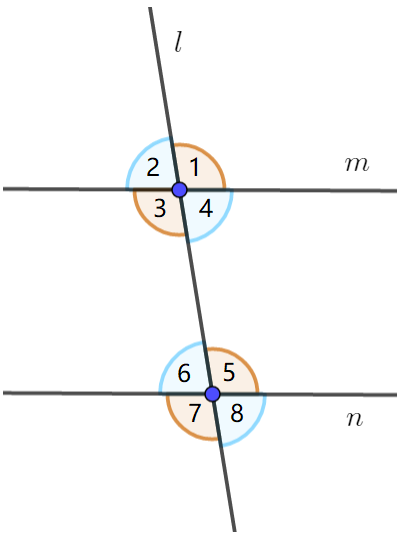
\includegraphics[width=0.4\textwidth]{三线八角.png}
% \end{wrapfigure}

% 最后我们证明同位角相等和平行线的关系。
% \begin{tm}\label{tm:3-0-4}
%     如右图,设直线$l$与两条直线$m,n$相交于两点。同位角$\angle 1$和$\angle 5$相等,当且仅当$m,n$平行。
% \end{tm}
% \begin{proof2}

% \end{proof2}


\end{document}